\documentclass[bibtotoc,oneside]{scrbook}

\usepackage[a4paper]{geometry}
\usepackage[english]{babel}
\usepackage[utf8]{inputenc}
\usepackage{graphicx}
\usepackage{url}
\usepackage{hyperref}
\usepackage{listings, color}
\usepackage{scrpage2}					% header and footer line
\usepackage{longtable}
\usepackage{subfigure}
\usepackage[acronym, nonumberlist, toc]{glossaries}

\usepackage[autostyle]{csquotes}
\usepackage{biblatex}
\nocite{*}

\usepackage{algpseudocode}

\lstset{
    frame=single,
    showspaces=false,
    language=[Objective]Caml
}

\usepackage[nottoc]{tocbibind}

\usepackage{xcolor}
\hypersetup{
    colorlinks,
    linkcolor={red!50!black},
    citecolor={blue!50!black},
    urlcolor={blue!80!black}
}

\usepackage{enumitem}
\usepackage{calc}
\SetLabelAlign{parright}{\parbox[t]{\labelwidth}{\raggedleft#1}}

\usepackage{amssymb}

% header and footer line - no header & footer line on pages where a new chapter starts
\pagestyle{scrheadings}

\graphicspath{{./img/}}

\makenoidxglossaries
\newglossaryentry{computer}
{
    name=computer,
        description={is a programmable machine that receives input,
            stores and manipulates data, and provides
                output in a useful format}
}

\newglossaryentry{potato}{name={potato},plural={potatoes},
description={starchy tuber}}
\newglossaryentry{cabbage}{name={cabbage},
description={vegetable with thick green or purple leaves}}
\newglossaryentry{carrot}{name={carrot},
description={orange root}}

%\newacronym{api}{API}{Application Programming Interface }

%%% The glossary entry the acronym links to   
\newglossaryentry{api}{name={API},
    description={An Application Programming Interface (API) is a particular set
    of rules and specifications that a software program can follow to access and
    make use of the services and resources provided by another particular software
    program that implements that API}}

%refactor definitions ofc

%Native code/machine code
%IR Intermediary Representation
%Optimization
%Backtrace
%Inlining
%Object file
%Runtime
%Binding
%Multi-pass compiler?

%In computing, a binding from a programming language to a library or operating system service is an application programming interface (API) providing glue code to use that library or service in a particular programming language.

%functional interface to second library in a different programming language


    %%% define the acronym and use the see= option
    %\newglossaryentry{api}{type=\acronymtype, name={API}, description={Application
    %Programming Interface}, first={Application
    %Programming Interface (API)\glsadd{apig}}, see=[Glossary:]{apig}}


\bibliography{./bib/references}

\usepackage{pifont}

\usepackage{afterpage}

\newcommand*\tick{\item[\ding{51}]}
\newcommand*\fail{\item[\ding{55}]}

\newcommand*\pro{\item[$+$]}
\newcommand*\con{\item[$-$]}

\newcommand*\BitAnd{\mathrel{\&}}
\newcommand*\BitOr{\mathrel{|}}
\newcommand*\ShiftLeft{\ll}
\newcommand*\ShiftRight{\gg}
\newcommand*\BitNeg{\ensuremath{\mathord{\sim}}}

\usepackage{tikz}
\usetikzlibrary{positioning}
\usetikzlibrary{shadows,arrows}
\tikzstyle{line} = [draw, thick, color=black!50, -latex']

\definecolor{mybluei}{RGB}{124,156,205}
\definecolor{myblueii}{RGB}{73,121,193}
\definecolor{mygreen}{RGB}{202,217,126}
\definecolor{mypink}{RGB}{233,198,235}

\begin{document}

% ---------------------------------------------------------------
\frontmatter
    \thispagestyle{empty}
\begin{center}

\vspace*{1.4cm}
{\LARGE \textbf{OCaml native debugging with LLDB}}

\begin{figure}
    \centering
    \subfigure{\includegraphics[width=60mm]{ocamlpro-logo}}
    \hspace{1em}
    \hfill
    \subfigure{\includegraphics[width=60mm]{upmc}}
\end{figure}

\vspace*{1.0cm}

{\LARGE Internship Report - Master's Thesis}\\

\vspace{1.0cm}
{\LARGE \textbf{Université Pierre et Marie Curie}}\\
\vspace*{0.3cm}
{\LARGE \textbf{Paris, France}}\\
\vspace*{1.0cm}
{\LARGE Elias BOUTALEB}
\\
\vspace*{0.5cm}
\today
\vspace*{1.0cm}

Supervised by\\
    Jacques MALENFANT (UPMC/LIP6)\\
    Fabrice LE FESSANT (OCamlPro)\\
\vspace*{0.5cm}
\vspace{3cm}


\end{center}


   	\thispagestyle{empty}

    %\thispagestyle{empty}
\vspace*{1.0cm}

\begin{center}
    \textbf{Abstract}
\end{center}

\vspace*{0.5cm}

\noindent
In your thesis you should try to explain as much as possible with the help of images.
\\
\\
The abstract is the most important part of your thesis. Take your time to write it as good as possible. Abstract should have no more than one page. It is normal to rewrite the abstract again and again, so  probaly you won't write the final abstract before the last week of due-date. Before submitting your thesis you should give at least the abstract, the introduction and the conclusion to a native english speaker. It is likely that almost no one will read your thesis as a whole but most people will read the abstract, the introduction and the conclusion.
\\
\\
Start with some introductionary lines, followed by some words why your topic is relevant and why your solution is needed concluding with 'what I have done'. Don't use too many buzzwords. The abstract may also be read by people who are not familiar with your topic.

    %\thispagestyle{empty}
    %\cleardoublepage

    \tableofcontents
    \thispagestyle{empty}

% --------------------------------------------------------------
\mainmatter % comment single chapters for faster compilation
    \chapter{Introduction\label{cha:chapter1}}

There are things to be aware of when dealing with machine native code
the instructions themselves do not retain any information about /concerning the abstractions in the
original source code, because the CPU does not need it

backend compiler passes
%reorganize and reposition instructions
furthermore, compiler optimizations can move, add and transform instructions in such a way that it might not be possible
to identify which source code statement correpsond to a particular/specific set of machine instruction

hence, compilation of a program to native code involve a huge loss of information
information that is usually collected by compilers and bundled with binaries/object files in the form of
debugging information for debuggers.

\section{Motivation\label{sec:moti}}

necessary to debug native code, in cases where a bug might appear only in a optimized binary/program
%(if inline assembly code is inserted manually by a developer e.g)
easier to debug unoptimized, but inspecting assembly code instruction and memory becomes a tedious task in a large program

there is for now no lasting? comprehensive? definitive? solution for debugging OCaml native code
partial effort was made, bare minimum is here (backtrace support, partial step by step into function entry points and function calls)

no variable inspection, main debuggers unaware of the OCaml native runtime management of values
moslty assembly/ raw memory view, arcane knowledge of target architecture, not available to every developper

\section{Objectives\label{sec:objective}}
The work presented here aims to address
Improve debugging support for OCaml native compiled code
Enhance the debugging experience

diminish cognitive strain on devs

targeting developers lacking knowledge of the target architecture

\section{Scope\label{sec:scope}}

Find a way to generate more debugging information (which info)
Store it in a adequate/fitting debug data format

Improve a prototype of native debugger based on LLDB

The OCamlPro company
Internship timeline (every forthnight)

\section{Outline\label{sec:outline}}

\textbf{Chapter \ref{cha:chapter2}} is usually termed 'Related Work', 'State of the Art' or 'Fundamentals'. Here you will describe relevant technologies and standards related to your topic. What did other scientists propose regarding your topic? This chapter makes about 20-30 percent of the complete thesis.
\\
The DWARF standard
The DWARF format
Example
The ocplib-dwarf library
\\
\textbf{Chapter \ref{cha:chapter3}} analyzes the requirements for your component. This chapter will have 5-10 pages.
\\
The OCaml native toolchain
hl architecture, compilation process

debug loc
dwarf
types
for each, what effect is achieved, tradeoffs
\\
\textbf{Chapter \ref{cha:chapter4}} is usually termed 'Concept', 'Design' or 'Model'. Here you describe your approach, give a high-level description to the architectural structure and to the single components that your solution consists of. Use structured images and UML diagrams for explanation. This chapter will have a volume of 20-30 percent of your thesis.
\\
The OCaml native runtime
LLDB (API)
ocp(lib)-lldb (hl archi)

additions to LLDB and ocp-lldb
\\
\textbf{Chapter \ref{cha:chapter5}} describes the implementation part of your work. Don't explain every code detail but emphasize important aspects of your implementation. This chapter will have a volume of 15-20 percent of your thesis.
\\

\\
\textbf{Chapter \ref{cha:chapter6}} is usually termed 'Evaluation' or 'Validation'. How did you test it? In which environment? How does it scale? Measurements, tests, screenshots. This chapter will have a volume of 10-15 percent of your thesis.
\\
How does it fare?
\\
\textbf{Chapter \ref{cha:chapter7}} summarizes the thesis, describes the problems that occurred and gives an outlook about future work. Should have about 4-6 pages.

&& Améliorations
&& Extensions
Work being done in same direction

    \chapter{Introduction to the DWARF format\label{cha:chapter2}}

To establish correspondence between high-level source code and low-level machine code, one wants to
\begin{itemize}
    \item  collect all information generated im the compiling process
    \item  and represent that information in a suitable format usable by debuggers, concisely and compactly
\end{itemize}

DWARF is a debugging data format allowing support for source level debugging
it has with the following characteristics:

It is widely used today
it is language agnostic, independent of compiler tooling (linker/assembler),
target architecture and debuggers.
It is somewhat object file agnostic, although mostly associated with the ELF object file format.

it is standardized, meaning it has specifications and norms codified into
a formal document.
A commitee oversees additions/extensions to the standard to follow the
appearance of programming languages and their evolution

\section{Important DWARF sections and their contents}

%\begin{description}[leftmargin=!,labelwidth=\widthof{\bfseries .debug\_abbrev}]
\begin{description}[labelwidth=\widthof{\bfseries .debug\_abbrev},align=parright]
    \item[.debug\_abbrev] Abbreviations used to decode the .debug\_info section
    \item[.debug\_frame] Call frame information table
    \item[.debug\_info] Core DWARF data section
    \item[.debug\_line] Line number information table
    \item[.debug\_loc] Location lists for runtime location of variables/parameters
    \item[.debug\_str] String table reference in .debug\_info
\end{description}

\section{Storage}

The debugging information is stored in sections in the object file.

In the separate compilation process, the DWARF sections of each object file are
put together in their common corresponding section in the final binary

Binary data format

Multiple techniques are used to reduce the size of the debugging information:

LEB128 is a variable length compression encoding
it allows for encoding of signed and unsigned integers of arbitrary size.
Used in DWARF to encode values of various fields (like attributes)

Some of the section tables can become quite large.
In order to save space, those tables are encoded as bytecode instructions to be executed by state machines to obtain their fully expanded form

\section{Structure}

\subsection{Debugging information entry}

In DWARF, the base entity manipulated is called an debugging information entry, or DIE.
A DIE is made of a tag specifying what language construct it describes and a list of attributes giving more details concerning that construct.

A DIE tag can designate for example entities such as:
\begin{description}
    \item[DW\_TAG\_subprogram] — A subroutine/function
    \item[DW\_TAG\_variable] — A variable
    \item[DW\_TAG\_formal\_parameter] — An argument within function parameters
    \item[DW\_TAG\_lexical\_block] - Define lexical scoping of local variables
    \item[DW\_TAG\_base\_type] - Primitive type not defined in terms of other
        types
\end{description}

An attribute is a name/value couple.
The name attribute indicates what the value represents (name, absolute address,
bytecode, offset, string, integer) and what class of values are supported
It is hence possible for attributes values to reference other DIEs and DWARF sections.

\begin{description}
    \item[DW\_AT\_name] String naming the designated DIE
    \item[DW\_AT\_stmt\_list] Offset referencing a location list
    \item[DW\_AT\_type] Reference to a type DIE
    \item[DW\_AT\_low\_pc] address of the first machine instruction
    \item[DW\_AT\_high\_pc] address or offset/constant of the first location past the last instruction
\end{description}

A DIE can be nested in another parent DIE, have siblings and children,
can be represented as a tree with an arbitrary number of children

The subprogram DIE owns DIEs describing the subprogram.

\subsection{Compilation unit}

It designates two entities :

each separately compiled source file is considered as a compilation unit
the root of a DIE tree that starts the DWARF data for the source file it represents
It contains general information about the compilation,
such as the programming language, the compiler version used, source file name, flags

\section{Example}

\section{The ocplib-dwarf library}

it is a library written in OCaml that reads and prints DWARF data in a human readable format similar to objdump
made in a effort to learn and comprehend the DWARF format during the internship.

DWARF emission writing and editing features are not yet implemented
not sure it is useful, as this task is left to compilers

high level desc

%todo prepare a schema

driver with command line option handling

offers abstraction that allow DWARF data manipulation
can visualize the DIE tree structure in debug\_info in DOT format using graphviz
to emulate mutable trees, a zipper library was implemented

utility functions for reading binary data

section parsing implemented accordingly to the DWARF4 standard by its own module
printing module operates on DWARF data structures in ocaml

hexadecimal view available for debugging purposes


    \chapter{The OCaml native compiler\label{cha:chapter3}}

The OCaml language support multiple programming paradigms:
\begin{itemize}
    \item functional programming style, that consists mostly of pure computations that always
        evaluate to the same value across different executions for the same arguments
        and do not produce side effects.
    \item in contrast, in the imperative programming style,
        use of assignments to mutable variables can result in side effects
        where the return value of a routine may change across multiple executions,
        modify some state in the program or perform I/O operations
        such as writing to a file.
\end{itemize}

In both styles, stepping through function calls is fine, regardless of whether
they are pure or not.
However, in the case of side-effecting functions, one must be vary of the order of
evaluation of arguments, as they may affect the return value.

Moreover, it may not make much sense to source debug functional constructs
the same way one would with with equivalent imperative constructs.
The use of map and filter functions, first class functions and
partial function application come to mind.
Nonetheless, bugs bound to those constructs are usually programming
logic errors, not run-time or compiler errors.

\section{The native compilation process}

A OCaml source program goes through multiple passes/transformations:

\begin{description}
    \item[lexing - lexical analysis]
        split the program from a sequence of characters into a sequence of
        tokens, contain file and line location information.

    \item[parsetree - syntactic analysis]
        check whether the program as a sequence of tokens is gramatically valid, and if so
        construct an abstract syntax tree.

    \item[typedtree - semantic analysis]
        perform type inference and checking, annotate AST with type information

    \item[lambda]
        AST with pattern matching translation,
        % to if and switch constructs,
        elimination of classes and modules,
        discards type information and most of location information,
        %maps the source code to runtime memory model,
        generates unique names for identifiers by appending a number stamp to them
        (variable shadowing)

    \item[clambda]
        closure conversion (to lexical blocks?), inlining, constant propagation
        and folding

    \item[cmm]
        primitives conversion % high level to low lvl operations

    \item[mach]
        allocation merging, register liveness analysis, register spilling and allocation

    \item[linearize]
        the AST becomes a sequence of pseudo machine code instructions

    \item[emit] assembly code generation

    \item[assembling and linking final binary]
\end{description}

%\afterpage{%
\afterpage{\clearpage}
\begin{figure}
  \centering
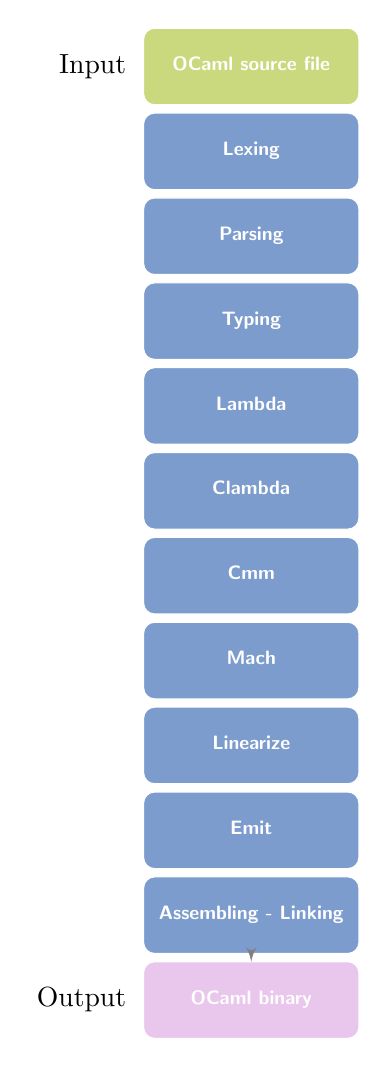
\begin{tikzpicture}[node distance=3pt,outer sep=0pt,
blueb/.style={
  draw=white,
  fill=mybluei,
  rounded corners,
  text width=2.5cm,
  font={\scriptsize\sffamily\bfseries\color{white}},
  align=center,
  text height=12pt,
  text depth=9pt},
greenb/.style={blueb,fill=mygreen},
]
\node[blueb, fill=mygreen] (prog) {OCaml source file};
\node[left=of prog] (i) {Input};
\node[blueb, below=of prog] (lex) {Lexing};
\node[blueb, below=of lex] (par) {Parsing};
\node[blueb, below=of par] (typ) {Typing};
\node[blueb, below=of typ] (lam) {Lambda};
\node[blueb, below=of lam] (clam) {Clambda};
\node[blueb, below=of clam] (cmm) {Cmm};
\node[blueb, below=of cmm] (mac) {Mach};
\node[blueb, below=of mac] (lin) {Linearize};
\node[blueb,below=of lin] (cgen) {Emit};
\node[blueb,below=of cgen] (asm) {Assembling - Linking};
\node[blueb,fill=mypink,below=of asm] (bin) {OCaml binary};
\node[left=of bin] (o) {Output};

\path [line] (asm.south) -- node [above] {} (bin) ;
\end{tikzpicture}
\end{figure}

\afterpage{\clearpage}
%\clearpage
%}

\section{Additions to the compiler}

\subsection{Location information}

Let us define first what a debugging event is, quoting the OCaml manual:

\begin{quotation}
    Events are “interesting” locations in the source code, corresponding to the
    beginning or end of evaluation of “interesting” sub-expressions. Events are
    the unit of single-stepping (stepping goes to the next or previous event
    encountered in the program execution). Also, breakpoints can only be set at
    events. Thus, events play the role of line numbers in debuggers for
    conventional languages. \autocite{events}
\end{quotation}

Those events are inserted in OCaml bytecode programs for use with the source-level bytecode
debugger \textit{ocamldebug}. \\

Among the debugging information to be added, line information is important,
both for stepping into the source program statement by statement,
and also for setting breakpoints by file and line number.

The idea here is to propagate the location information contained in those events
through the native code backend, by wrapping all IR nodes into a record
containing the node and a field with location information from the debugging
event.

\begin{lstlisting}
type t = {
  dinfo_file: string;
  dinfo_line: int;
  dinfo_char_start: int;
  dinfo_char_end: int
}

type 'a expression = {
  exp: 'a;
  dbg: t;
}
\end{lstlisting}

This has been done for every native backend pass all the way up to the linearize
pass, whose instruction record that already contains such a field.

Then, location information was attached to some particular constructs:

\begin{itemize}
    \item integers - as empty list [] and None from the option type represented as integers
        useful in pattern matching as well
    \item primitives - in particular :

%- explain what a primitive is, what it is responsible for

%prim operations mirroring bytecode instructions maybe?
%may refer to external C function
%assignments, allocation, comparisons, string/float/integer/boolean operations,
%boxed/unboxed
        \begin{itemize}
            \item
                Test comparisons in if-then-else statements
                since primitives have location information, it is possible to
                stop at the comparison test.
                Pattern matching can take advantage of this too, since they are compiled into
                if and switches constructs at the lambda pass.
            \item
                setfield primitive - responsible for mutable assignments of variables, mutable
                fields in records and non-constant let assignments
            \item
                allocation - before initializing any boxed values
        \end{itemize}
\end{itemize}

At the code generation step, the code emitter uses two notable debugging
assembly directives, specific to the GNU assembler as it is used in the
compilation process:

%https://sourceware.org/binutils/docs-2.26/as/Loc.html
%https://sourceware.org/binutils/docs-2.26/as/File.html

\begin{itemize}
    \item .file fileno filename : assigning a positive integer to a filename
    \item .loc fileno lineno [column] [options] : add a row to the .debug\_line
        line information matrix for the current compilation unit, map a source
        file and line number to the assembly instructions that follow
\end{itemize}

Avantages and disadvantages:

\begin{itemize}
\fail
Heavy modifications on the backend
% huge patch when trying to add a debugging field to every IR node
% languages des passes backend natif n'a pas prevu pour l'adjonction d'info de debug
\fail lack of accuracy, loss of information still occuring as code is still expanded and transformed
%\item Valeurs disponibles pas toujours cohérentes
% csq du manque de precision
\tick Although the initial work require a bug code patch, further modifications
and information propagation becomes easier, as opposed to add a location field
to every construct record definition
\tick Can step more naturraly into imperative constructs
(pattern matching/branching, assignments)
\end{itemize}

\subsection{Runtime location of variables}
%calling conventions differ from C
When about to call OCaml functions, arguments are passed in registers first
and remainders on the stack.
The OCaml runtime tries to reuse registers as much as it can, variables
are spilled on the stack if no registers are available.
Callee functions can clobber their callers' arguments.

Add 2 passes into the backend: available\_regs and available\_ranges
using forward data-flow analysis operating on Mach IR, can be traversed like
a \gls{cfg}
intraprocedural DFA

available\_regs overview :
takes a function expressed in Mach code as input
return Mach code with each ins annotated with set of `registers` identifiers
augmented with a set of available variables for each instruction

whose value can be accessed (hence available) by a debugger at runtime

The data-flow equations used for a given instruction
\[
    \textit{out}_{b} = \bigcup_{s \in succ_{b}} \textit{in}_{s}
\]
\[
    \textit{in}_{b} = (\textit{out}_{b} - \textit{kill}_{b}) \cup \textit{gen}_{b}
\]
in : set of symbolic registers used by a particular variable right before
current instruction gets executed

kill : set of clobbered/overwritten reg variables considered as unavailable because of the nature of the
current instruction
%out(b) = 0
%for s in succ(b)
  %out(b) = out(b) or in(s)
  %in(b) = (out(b) and not kill(b)) or gen(b)
available\_ranges:
operates over Linearize function declaration annotated with available\_regs pass
calculates for each variable/ identifier used in target function the memory
addresses ranges where its content can be inspected, and for each range, the
place where the content can be accessed (in registers or on the stack)

available before

sub-range : starting instruction * starting label * ending label * symbolic
register
range : list of sub-ranges * minimal/lowest position/label * highest label
such as no overlaps between subranges

%new instruction_descr in linearize.ml

%- Lavailable_subranges of int option ref
%- Lprologue

ranges : map from identifiers to a range

process each identifer found in a Linearize function declaration

and insert labels to delimit/demarcate variable availability in the Linearize
fundecl, hence it modifies it

with information collected beforehand by available\_regs

\begin{algorithmic}[1]
    \If{some condition is true}
    \State do some processing
    \ElsIf{some other condition is true}
    \State do some different processing
    \ElsIf{some even more bizarre condition is met}
    \State do something else
    \Else
    \State do the default actions
    \EndIf
\end{algorithmic}


unique identifier with unique stamp is generated in cases variable shadowing overwrites former value

not every value binding is captured becaused of constant folding, static
constant stored and loaded in register instead

as a consequence of the lack of precision from the events,
location information directives are not put at the
most suitable assembly instruction, and values might not be updated when they should
at some point in the source and vice versa

\subsection{DWARF emitter}

using the labels generated by available\_ranges, calculates offset differences
betweens label subranges to populate the .debug\_loc section

populate the  .debug\_info as well with function/routine DIEs

no type information encoded in the DWARF, will be handled later separately.

output each variable DIE in its own, separate lexical block with specific range
no nesting of lexical block

DWARF information can be added to the binary using the `-gdwarf` compiler option flag.

The DWARF emitter and runtime location of variables features are both credited to
Mark Shinwell from Jane Street Europe.

Minor adjustments and bug fixes were made for both to work properly with the initial codebase.

\subsection{Type information}

We can now determine where a particular variable value is located in memory, but
we do not know how to interpret it. Type information of variables is necessary
at this point, but by the time the compilation process reach its latter end,
type information is already discarded. \\

The OCaml compiler offers the option of exporting the \gls{ast} annotated with type
information at the typedtree pass into a file with the cmt extension (using the
flag -bin-annot). \\

Typed \gls{ast} is serialized into the binary instead of a separate file.

It is more practical/easier to manipulate, but comes at the cost of a bigger binary
size.
It can be added to the binary using the `-dvb` compiler flag.\\

That information will be used later to build a symbol table for use in the
ocp-lldb native debugger.


    \chapter{Interfacing with LLDB\label{cha:chapter4}}

%todo refactor

We developed the first prototype of a native debugger for OCaml, based on the LLDB debugging framework on top of LLVM. For that, we first generated a full OCaml binding for the LLDB library, by parsing the C++ headers of the libraries and automatically generating OCaml and C++ stubs. We were then able to use the OCaml binding to develop several tools, ranging from a simple tool that displays the internal GC information of a finished OCaml application, to an almost complete debugger, which displays OCaml values using runtime type information added for memory profiling.

The OCaml native runtime system
LLDB (API)
ocp(lib)-lldb (hl archi)

additions to LLDB and ocp-lldb

\section{Introduction to LLDB}

LLDB\autocite{}
aims to be a modern source-level debugger, modular plug-in arch (for obj file
format, prog lang support, symbol files, disasm, specific hosts/targets), reusable components, public
C++ API interface to library for access to and control of debugger instances,

python bindings,
can interact with debug instances and build applications that provide debugging features

 C, Objective-C, C++ Swift

part of the llvm project (collection of compiler tools with reusable components)
including clang compiler prog lang frontend, and llvm middle end IR and code gen backends
for multiple architectures, machine dependent? target

several compiler frontends for support of mult prog languages (clang, rust)


Figure \ref{fig:aliceandbob} illustrates the situation between Alice and Bob. (sequence diagram from www.websequencediagrams.com)


\subsection{LLDB OCaml language plugin}

at this point, a OCaml program compiled with a compiler and modifications
presented previously contains more information relevant to debugging than before

more places where to set a breakpoint in the program
runtime location of variables
type information

however, the information provided by 2 and 3 cannot be used directly as it is yet:
using LLDB directly


current versions of LLDB arent aware of OCaml
Ocaml binary mixing C with OCaml assembly code
LLDB bindings doesnt allow access to the DWARF data nor name symbol demangling

however, it is now possible for LLDb to support other languages/ debug binaries
written in different programming languages
% depuis un peu moins d'un an, chgmts faits a LLDB pour pouvoir supporter d'autres languages que ceux supportes par clang
% il suffit d'ecrire des classes impl certaines interfaces
% ajouter le language cible dans un enum

% eventuellement pouvoir evaluer expr dans ce language
% pretty printing des valeurs et typage dynamique, ptes statiques ou dyn du language
facilities for evaluating language expressions
express static dynamic properties of the language

among the addition done to LLDB

barebones OCaml LLDB plugin

custom DWARF parser

minimal type system, data structures used to represent OCaml types may
    change from one version to another, it might not be maintainable to update
    the LLDB plugin at each release
    backwards compatibility concerns
    thus, all values are to be considered as 64-bits integers, and their
    interpretation according to their types will be left to ocp-lldb

    does symbol demangling as well

    mangled ocaml symbol of the form
    make demangled form available for easier breakpoint setting

\section{ocp-lldb}

%todo ocp-lldb architecture

\begin{figure}[htb]
  \centering
  \includegraphics[width=9cm]{uml_seq_example.png}\\
  \caption{Alice and Bob}
  \label{fig:aliceandbob}
\end{figure}

ocplib-lldb \\

taking advantage of the OCaml compiler frontend as a library
allowing use of the lexer and parser and typing facilities, esp
useful when operating over parsetree/typedtree representation

used to build symbol table mapping identifiers in the prog to their type
for runtime value interpretation

can generate an OCaml binding to LLDB API

parse header files in LLDB
most classes and methods of the API are supported, except static methods
access to C++ objects done through the OCaml FFI C interface

ocp-lldb

symbol table management :
read the serialized typed AST, iterate over it to extract a simpler tree
structure
then one can actually lookup the type associated with an identifier and display
its value accordingly

\section{Runtime memory representation of OCaml values}

\Glspl{boxed} are represented as a pointer to a block structure, made of a
header followed by data
header contains size of the block, and tag describing what type of data it
contains
add level of indirection / deref

to differentiate between pointers and integer values at runtime, the runtime
system uses a tagged pointer representation, the least significant bit of a
value is used as a tag : an OCaml integer is encoded as a 31 or 63-bit machine integer = $ (x \ShiftLeft 1) \BitOr 1 $
represented as 31/63-bit

integers of type int are not boxed, this bit will be set to one
pointers are word-aligned, this bit is always set to zero
(all pointers will be divisible by 4, which means they will always end with two
0 bits)

int, char are unboxed
unit, false, empty list [] as 0
true as 1

arrays, records, tuples -> header + array of values
records with floats fields, array of floats -> header + array of floats

variant types -> variants without paramter are unboxed ascending ints, non
constants variants with parameters are boxed

    Améliorations
Work left to do

Those additions were done and tested on a x86 64-bit system using Linux, on a
closed project fork of the OCaml compiler, including memory profiling facilities.

debugging events propagation specific to the clambda middle end

improvements brought by the original developer concerns mostly a
new, middle end, inlining compiler pass called flambda.

infinity of programs with combination of constructs to test whether they play
out nicely together

%case of if\_const\_int.ml: goes back in the source to perform assignment to the
%b variable somewhat makes sense, although counter intuitive

global values bindings/vars are unmangled and see below

Enhancements

value inconsistencies
addition of .loc directives due to debugging events propagation the compiler is not aware of
the address ranges variables are available at

the available\_ranges pass is not exempt of bugs either, still experimental

User experience/interface minor:
- no function name symbol displayed in the backtrace
- global variables becomes available/displayed only after second call to `frame variable`

- value identifiers inserted at the lambda pass (bound, clos, index for loop,
match), not present in cmt/typedtree
- make it possible to "coerce"/typecast value?

Extensions
Work being done in same direction

\chapter{Conclusion\label{cha:chapter5}}
The final chapter summarizes the thesis. The first subsection outlines the main ideas behind Component X and recapitulates the work steps. Issues that remained unsolved are then described. Finally the potential of the proposed solution and future work is surveyed in an outlook.

\section{Summary\label{sec:summary}}

Explain what you did during the last 6 month on 1 or 2 pages!
\\
\\
\noindent The work done can be summarized into the following work steps

\begin{itemize}
		\item Analysis of available technologies
		\vspace{-0.11in}
		\item Selection of 3 relevant services for implementation
		\vspace{-0.11in}
		\item Design and implementation of X on Windows
		\vspace{-0.11in}
		\item Design and implementation of X on mobile devices
		\vspace{-0.11in}
		\item Documentation based on X
		\vspace{-0.11in}
		\item Evaluation of the proposed solution
\end{itemize}

\section{Dissemination\label{sec:dissemination}}

Who uses your component or who will use it?

Developers, OCaml users, system programmers
without needing knowledge of target architecture

Industry projects, EU projects, open source...? Is it integrated into a larger environment? Did you publish any papers?

\section{Problems Encountered\label{sec:problems}}

Summarize the main problems. How did you solve them? Why didn't you solve them?

\section{Outlook\label{sec:outlook}}
%\item Systèmes visés: Linux x86 64 bits
%\item Plupart des outils encore non disponible au public
% en particulier le fork du compilateur avec support pour profiling memoire
% devrait etre mis a disposition au public dans un futur plus ou moins proche
Emission DWARF \autocite{libmond} \autocite{dwpr}
may be available for OCaml 4.05, still a prototype


LLDB plugin reached the LLDB codebase,
release for 4.0

other patches still have to be integrated, may depend on the final form of the
debugging features

work done on ocp-lldb and ocplib-dwarf has been submitted
awaiting integration to typerex-binutils, reimplementation of the binutils tools
in OCaml and typerex-lldb

pull requests can be seen at

https://github.com/OCamlPro/typerex-lldb/pull/4
and
https://github.com/OCamlPro/typerex-binutils/pull/1

% compilateur reste a reste modifie en consequence
%\item ocp-lldb déjà disponible
%mais necessite fork avec memprof
%la branche sur laquelle je travaille necessite un autre fork encore avec mes ajouts

% Challenges et difficultes
%\item Augmenter le nombre de dbg events/locations
% chronophage car precision de methode naive + temps de compilation de la compiler suite
% comment faire composer les differents constructs ensemble
% Modifications entre debugger et compiler

ce que vous avez appris pendant votre stage que ce soit techniquement, méthodologiquement,
en termes de savoir-être en entreprise

I benefited in many ways from that internship:

I learned about inner workings of the OCaml toolchain,
I acquainted myself with multiple projects (OCaml, lldb) and contributed to their
codebases
I learned how debugging information is collected, synthetized and used in a debugger

learned to

weekly reporting of progress
time management between multiple related projects in parallel
compartimentation of related work in separate branchs using VCS


% ---------------------------------------------------------------
\backmatter
    \input{./misc/acronyms}
    \addchap{Annex}

\begin{appendix}

\lstset{
    numbers=left,
    basicstyle=\ttfamily\footnotesize,
    frame=single, % adds a frame around the code
    xleftmargin=3.4pt,
    xrightmargin=3.4pt
}

\lstinputlisting[caption=C program example,language=C, label={lst:tc}]{./t.c}

\begin{minipage}{\linewidth}
\lstinputlisting[firstline=22, lastline=51, label={lst:asm}, caption=x86\_64 assembly output of example program from line 4 to 11]{./t_ex.s}
\end{minipage}

\newpage

\begin{minipage}{\linewidth}
\lstinputlisting[lastline=52, caption=Output of .debug\_info section decoding from example program]{./t.dwarf}
\end{minipage}

\newpage

\begin{minipage}{\linewidth}
\lstinputlisting[firstline=53, firstnumber=53, label={lst:dwa}]{./t.dwarf}
\end{minipage}

\end{appendix}

\endinput

    \printbibliography

\end{document}
